\documentclass{article}
\usepackage[utf8]{inputenc}
\usepackage[english]{babel}
\usepackage{amsthm}
\usepackage{amssymb}
\usepackage{mathtools}
\usepackage{enumerate}
\newcommand\tab[1][1cm]{\hspace*{#1}}
\usepackage{graphicx}

\author{Kevin Martin\\ CIS675 - Syracuse University}
\title{Homework 3}

\newtheorem*{claim}{Question}
\renewcommand\qedsymbol{$\blacksquare$} 
\begin{document}
\maketitle
\begin{enumerate}
  \item Question 1
    \begin{enumerate}
        \item Table showing the intermediate distance values of all nodes at each iteration:\\
          \begin{figure}[h]
            \centering
          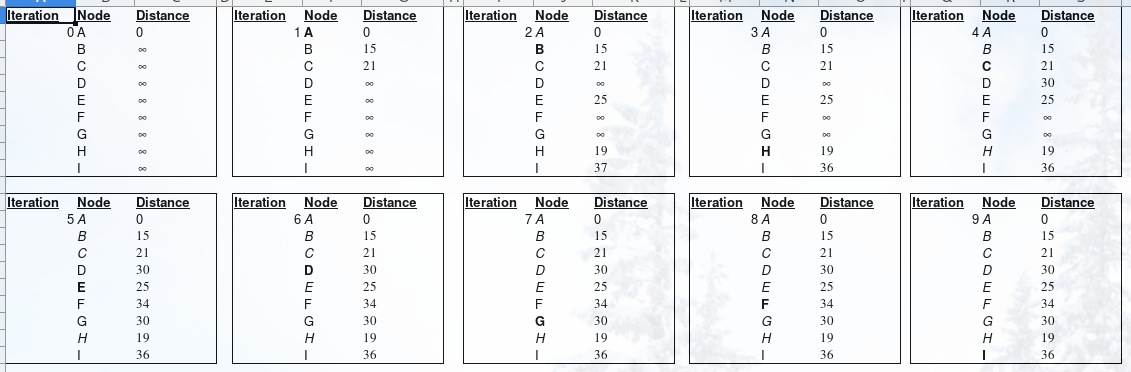
\includegraphics[scale=.4]{inttable3.png}
          \end{figure}


        \item Final shortest-path tree:\\
        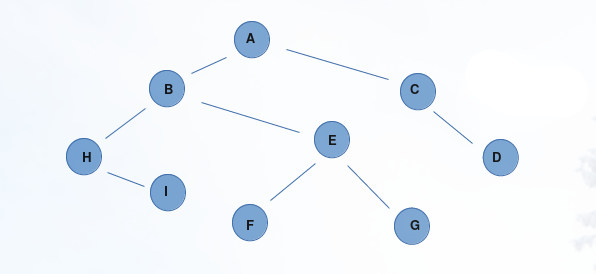
\includegraphics[scale=.7]{shorttree3.png}

        \item Adjaceny matrix representation with costs:\\
        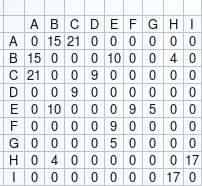
\includegraphics[scale=.75]{adjmatrix3.png}

        \item Adjaceny list representation with costs:\\
        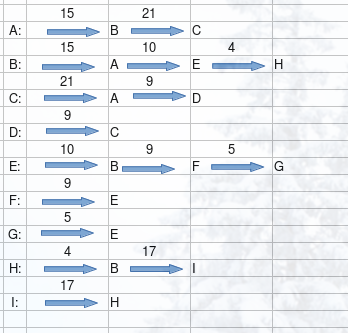
\includegraphics[scale=.5]{adjlist3.png}

    \end{enumerate}

    \item Question 2
      \begin{enumerate}
          \item The intermediate values of the delay array in each iteration, using Prim's algorithm:\\
            \begin{figure}[h]
              \centering
            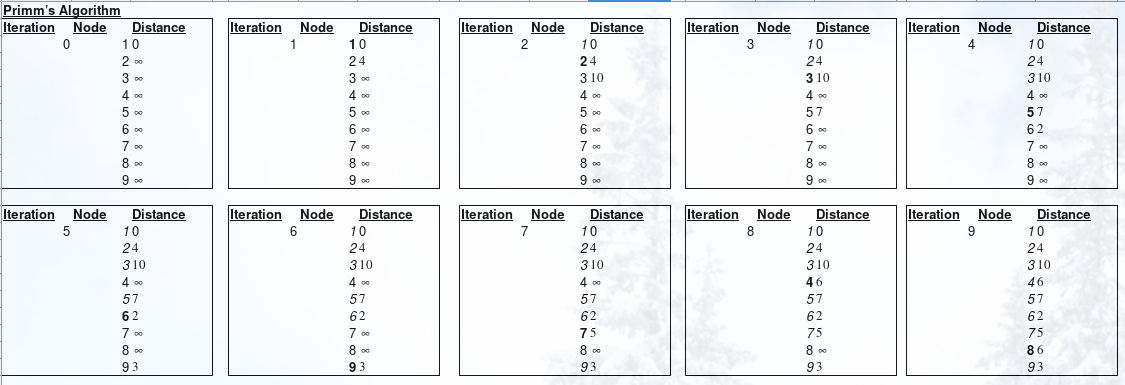
\includegraphics[scale=.40]{prim3.png}
            \end{figure}

          \item The disjoint-sets data structure at every intermediate stage, both regular intervals
            as well as assuming compression, using Kruskal's algorithm:\\
            \pagebreak
          \begin{figure}[h]
            \centering
          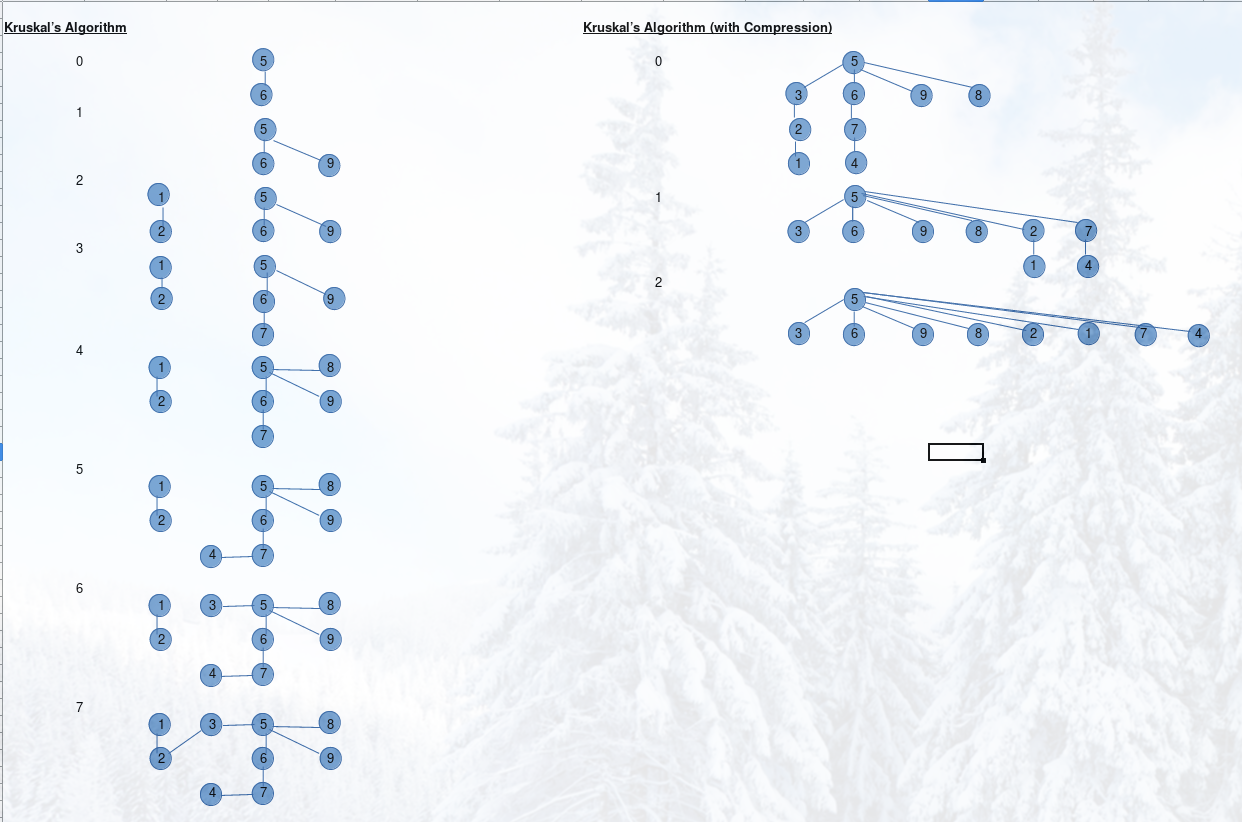
\includegraphics[scale=.36]{kruskal3.png}
          \end{figure}

        \end{enumerate}


  \item Question 3
      \begin{enumerate}
    \item \ Pseudocode for a greedy algorithm to compute optimal order and minimize wait time:\\\\
      Sort the service time in ascending order, and serve them in order of increasing scheduling
            times. \\
            Let n be the list of customers that need to be solved, with each time required $t_{i}$
            as the relevent index in the array:\\
      
      def greedySort(n [])\\
      sort(n); // in ascending order\\
      currentJob = n[1]\\
      for i = 1 to n:\\
          \tab currentJob = currentJob + $t_{i}$

             
    \item Claim: the running time of the proposed algorithm is $O(n logn)$
      \begin{proof}
      Sorting the list to get the algorithm started is where most of the time is required. Sorting a
        list of $n$ elements takes $O(nlogn)$ time. The rest of the algorithm can be completed in constant
        time, $O(1)$. Because the algorithm can be written as $c_{1}+(c_{1}+c_{2})+(c_{1}+c_{2}+...c_{n})
        \frac 1 n$, we can see that $c_{1}$ repeats itself the most times. As such, because it is the shortest
        time, then no other ordering could be correct. Therefore the greedy strategy holds true.

      \end{proof}

  \end{enumerate}

  \item Question 4
    \begin{enumerate}
      \item Optimum Huffman encoding (note: very unfavorable/inefficent outcome given the Fibonacci
        sequencing of the alphabet):\\
        \begin{figure}[h]
          \centering
        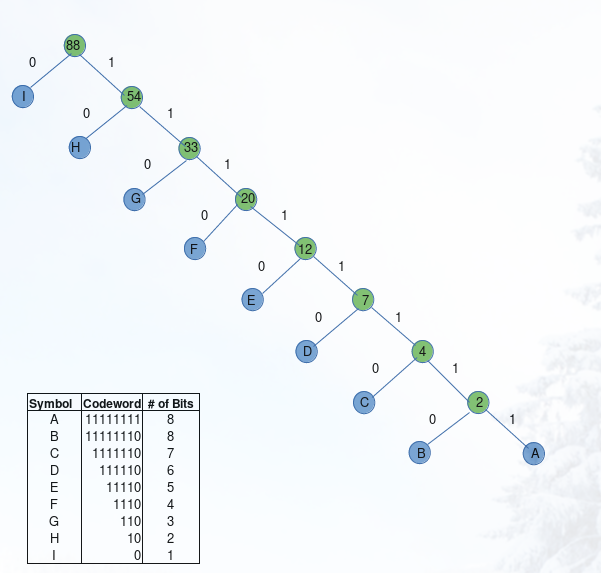
\includegraphics[scale=.65]{huffman3.png}
        \end{figure}

      \item The expected bits per letter are as follows:\\
        A: 8\\
        B: 8\\
        C: 7\\
        D: 6\\
        E: 5\\
        F: 4\\
        G: 3\\
        H: 2\\
        I: 1\\

    \end{enumerate}

  \item Question 5
      \begin{enumerate}
        \item To represent the situation as a linear problem, we formulate as follows, letting 
          $x_{1}$ be coffee mugs and $x_{2}$ be milk glasses:\\
          \tab Objective function \tab max $25x_{1}+20x_{2}$  \\
          \tab Constraints \tab \tab $20x_{1}+12x_{2} \leq 1800$  \\
          \tab \tab \tab \tab \tab $x_{1}/15+x_{2}/15 \leq 8$\\
          \tab \tab \tab \tab \tab $x_{1},x_{2} \geq 0$\\


        \item Graph of feasible region:
          \begin{figure}[h]
            \centering
        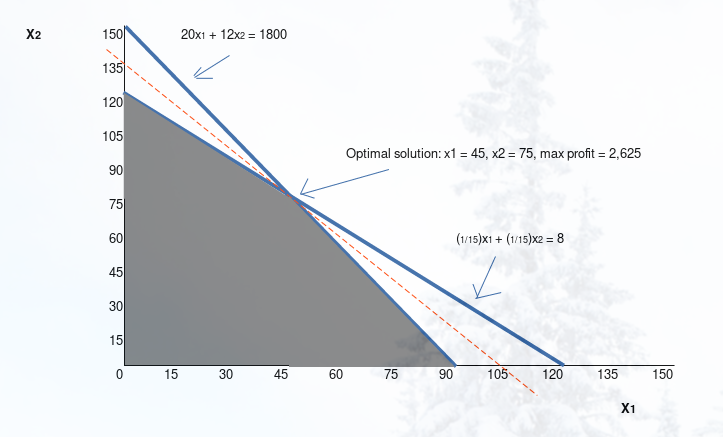
\includegraphics[scale=.6]{feasiblegraph3.png}
        \end{figure}
    
        \item The coordinates of all vertices of the feasible region are:\\
          (0, 0), (90, 0), (45, 75), (0, 120)

        \item The optimal product mix to maximize daily proift is:\\
          45 coffee mugs at \$ 25 each and 90 milk glasses at \$ 20 each, which 
          gives a total profit of \$2,625 per day.
          This is represented on the graph by the furthest out point on on the 
          feasible region, where the tangential dotted line intercepts the point
          (45, 75).

      \end{enumerate}

\end{enumerate}
\end{document}


